%!TEX program = pdflatex
\documentclass[UTF8]{ctexart}
\usepackage{amsmath}
\usepackage{booktabs}
\usepackage{lmodern}
\usepackage{geometry}
\usepackage{graphicx}
\ctexset{section={format={\Large\bfseries}}}
\geometry{a4paper,scale=0.8, centering}
\pagenumbering{arabic}

\title{\vspace{-1cm}CQF Exam One\\Portfolio and Risk Techniques}
\author{Kai Zheng}
\date{March 22, 2022}
\begin{document}
\maketitle

\section*{Question 1}
\begin{itemize}
	\item To solve for the weight in minimum variance portfolio with a target return m, we formulate
	      \begin{equation}\notag
		      \underset{w}{min}\frac{1}{2}w'\Sigma w
	      \end{equation}
	      subject to
	      \begin{equation}\label{1}
		      \begin{aligned}
			      w'\mu & = m \\
			      w'1   & = 1 \\
		      \end{aligned}
	      \end{equation}
	      The Lagrangian function is
	      \begin{equation}\label{2}
		      L(w,\lambda,\gamma) = \frac{1}{2}w'\Sigma w + \lambda(m-w'\mu) + \gamma(1-w'1)
	      \end{equation}
	      Its partial derivatives are
	      \begin{equation}\label{3}
		      \begin{aligned}
			      \frac{\partial L}{\partial w}(w,\lambda,\gamma) & = \Sigma w - \lambda \mu - \gamma1= 0
		      \end{aligned}
	      \end{equation}
	\item From (\ref{3}), the optimal weight solution has
	      \begin{equation}\label{4}
		      w^* = \Sigma^{-1}(\lambda\mu + \gamma 1)
	      \end{equation}
	      Bring this into (\ref{1}), we have
	      \begin{equation}\label{5}
		      \begin{cases}
			      \lambda = \frac{Am-B}{AC-B^2} \\
			      \gamma = \frac{C-Bm}{AC-B^2}
		      \end{cases}
	      \end{equation}
	      subject to
	      \begin{equation}\label{6}
		      \begin{cases}
			      A = 1'\Sigma^{-1} 1   \\
			      B = 1'\Sigma^{-1} \mu \\
			      C = \mu'\Sigma^{-1} \mu
		      \end{cases}
	      \end{equation}
	      Now we obtain $w^*$:
	      \begin{equation}\label{7}
		      w^* = \frac{1}{AC-B2}\Sigma^{-1}[(A\mu - B1)m + (C1 - B\mu)]
		      \vspace{2ex}
	      \end{equation}
	      Finally, calculate the optimal weight for the minimum variance portfolio and the standard deviation (please see the attachment for relevant codes). The summary tables is
	      \begin{table}[ht] \centering
		      \begin{tabular}{@{}lccccc@{}}
			      \toprule
			      \multicolumn{6}{c}{The allocation $w^*$ and portfolio risk $\sigma_\pi$}                 \\ \midrule
			            & $\sigma_\pi$ & \multicolumn{4}{c}{$w^*$}                                         \\
			      x1    & 0.05840091   & 0.78511066                & 0.05386419  & 0.13355472 & 0.02747042 \\
			      x1.25 & 0.0607102    & 0.81818944                & -0.00940302 & 0.17896585 & 0.01224773 \\
			      x1.5  & 0.06109091   & 0.87617647                & -0.14612952 & 0.32570145 & -0.0557484 \\ \bottomrule
		      \end{tabular}
	      \end{table}
	      \\
	      \\
	      \\
	      \\
	\item Generate 5,000 random allocations sets and satisfy $w'1 = 1$
	      \begin{figure}[ht]
		      \centering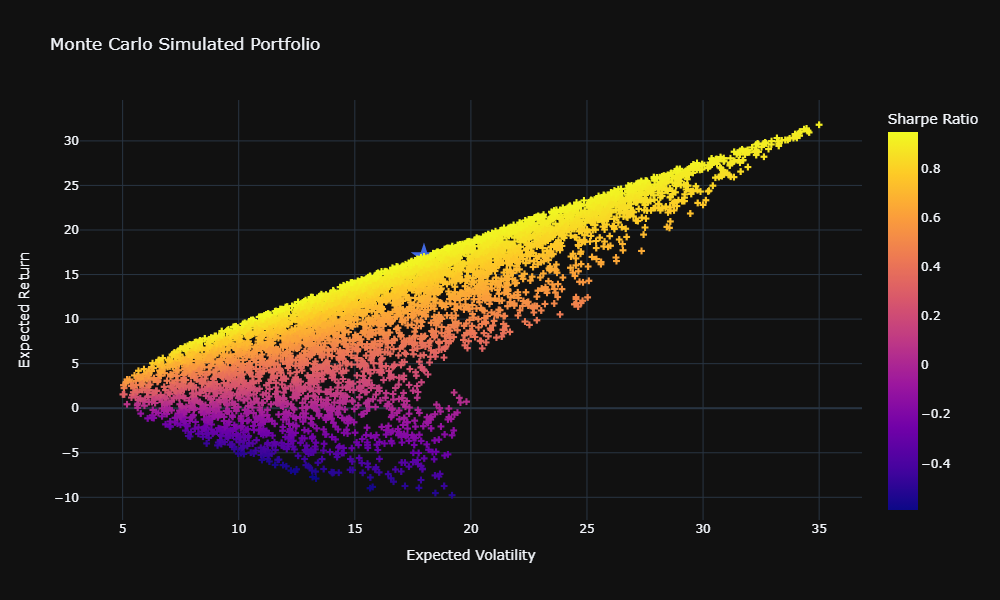
\includegraphics[scale=0.4]{1.3.png}
	      \end{figure}
\end{itemize}

\section*{Question 2}
\begin{itemize}
	\item To solve for risk minimization with N risky assets and a risk- free asset, we formulate
	      \begin{equation}\notag
		      \underset{w}{min}\frac{1}{2}w'\Sigma w
	      \end{equation}
	      subject to
	      \begin{equation}\label{8}
		      r + w'(\mu - r1) = m
	      \end{equation}
	      The Lagrangian function is
	      \begin{equation}\label{9}
		      L(w,\lambda) = \frac{1}{2}w'\Sigma w + \lambda(m - r - w'(\mu - r1))
	      \end{equation}
	      Its partial derivatives are
	      \begin{equation}\label{10}
		      \begin{aligned}
			      \frac{\partial L}{\partial w}(w,\lambda) & = \Sigma w - \lambda (\mu - r1) = 0
		      \end{aligned}
	      \end{equation}
	\item From (\ref{10}), the optimal weight solution has
	      \begin{equation}\label{11}
		      w^* = \Sigma^{-1}(\mu - r1)
	      \end{equation}
	      Substituting the value of $w^*$ into the constraint (\ref{8}), we solve for $\lambda$:
	      \begin{equation}\label{12}
		      \lambda = \frac{m - r}{(\mu - r1)'\Sigma^{-1}(\mu - r1)}
	      \end{equation}
	      Finally, we get $w^*$:
	      \begin{equation}\label{13}
		      w^* = \frac{(m - r)\Sigma^{-1}(\mu - r1)}{(\mu - r1)'\Sigma^{-1}(\mu - r1)}
	      \end{equation}
	      Because the tangency portfolio is fully invested in risky assets, then its asset allocation must satisfy the budget equation:
	      \begin{equation}\label{14}
		      1'w^* = 1
	      \end{equation}
	      We get:
	      \begin{equation}\label{15}
		      \begin{aligned}
			      w & = \frac{\lambda \Sigma^{-1}(\mu - r1)}{B - Ar} \\
		      \end{aligned}
	      \end{equation}
	      and
	      \begin{equation}\label{16}
		      \begin{aligned}
			      m      & = w'\mu             \\
			      \sigma & = \sqrt{w'\Sigma w}
		      \end{aligned}
	      \end{equation}
	      subject to
	      \begin{equation}\label{17}
		      \begin{cases}
			      A = 1'\Sigma^{-1} 1   \\
			      B = 1'\Sigma^{-1} \mu \\
		      \end{cases}
	      \end{equation}
	      The summary tables is (please see the attachment for relevant codes)
	      \begin{figure}[ht]
		      \centering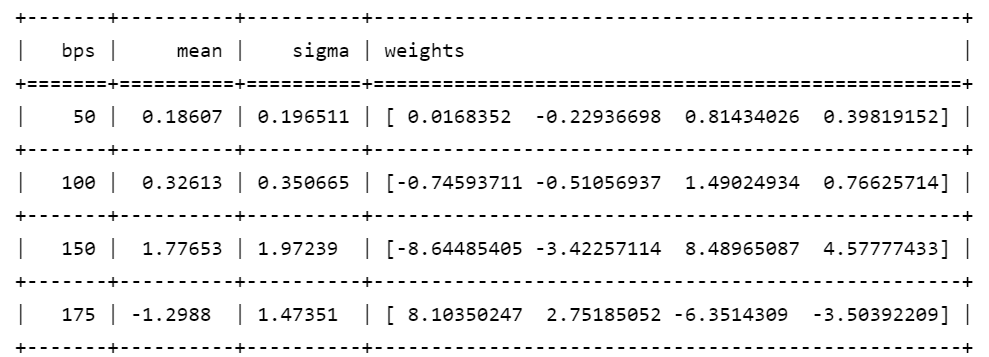
\includegraphics[scale=0.8]{2.2.png}
	      \end{figure}

	\item Plot the true Eficient Frontier by (0, $rf_{100bps}$) ($\sigma_{100bps}$, $\mu_{100bps}$), (0, $rf_{175bps}$) ($\sigma_{175bps}$, $\mu_{175bps}$) \\
	      \centering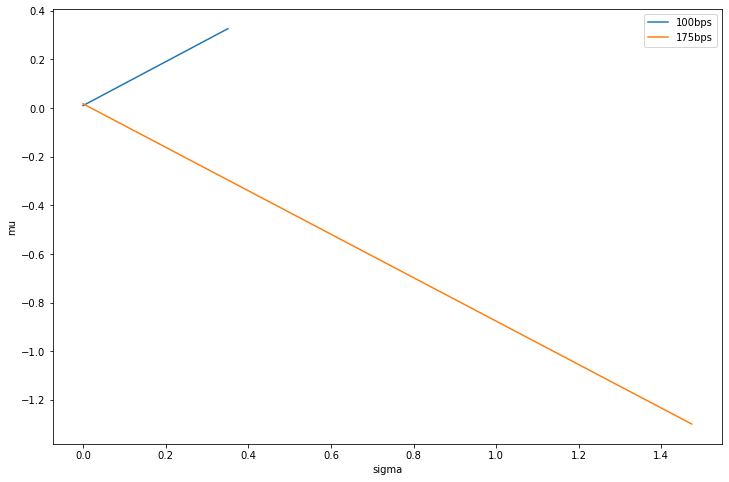
\includegraphics[scale=0.4]{2.3.png}
\end{itemize}

\section*{Question 3}
\begin{itemize}
	\item
	      a) the percentage of VaR breaches is $2.05\%$ \\
	      b) the number of consecutive breaches is 14 \\
	      c) provide a plot which clearly identifies breaches\\
	      \begin{figure}[ht]
		      \centering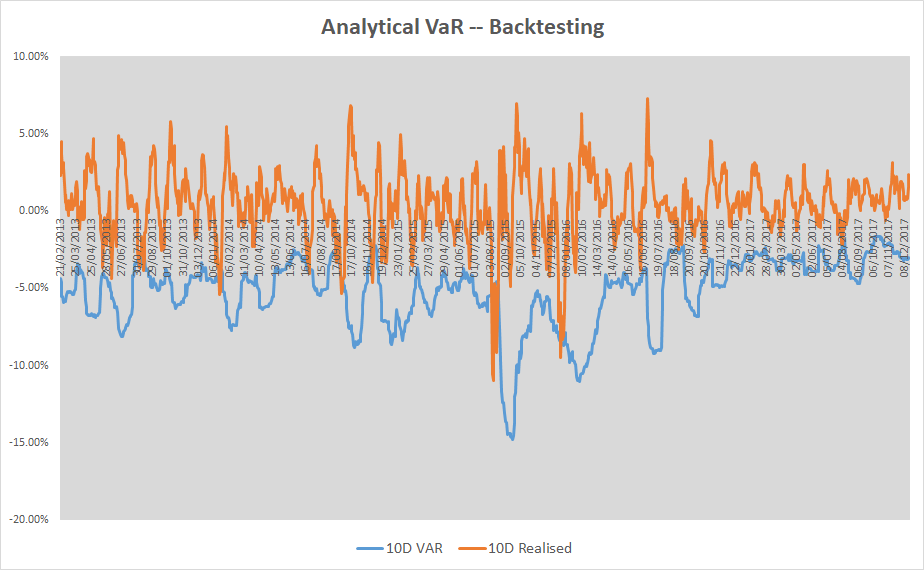
\includegraphics[scale=0.7]{3.1.png}
	      \end{figure}
	\item
	      a) the percentage of VaR breaches is $2.47\%$ \\
	      b) the number of consecutive breaches is 15 \\
	      c) provide a plot which clearly identifies breaches \\
	      \begin{figure}[ht]
		      \centering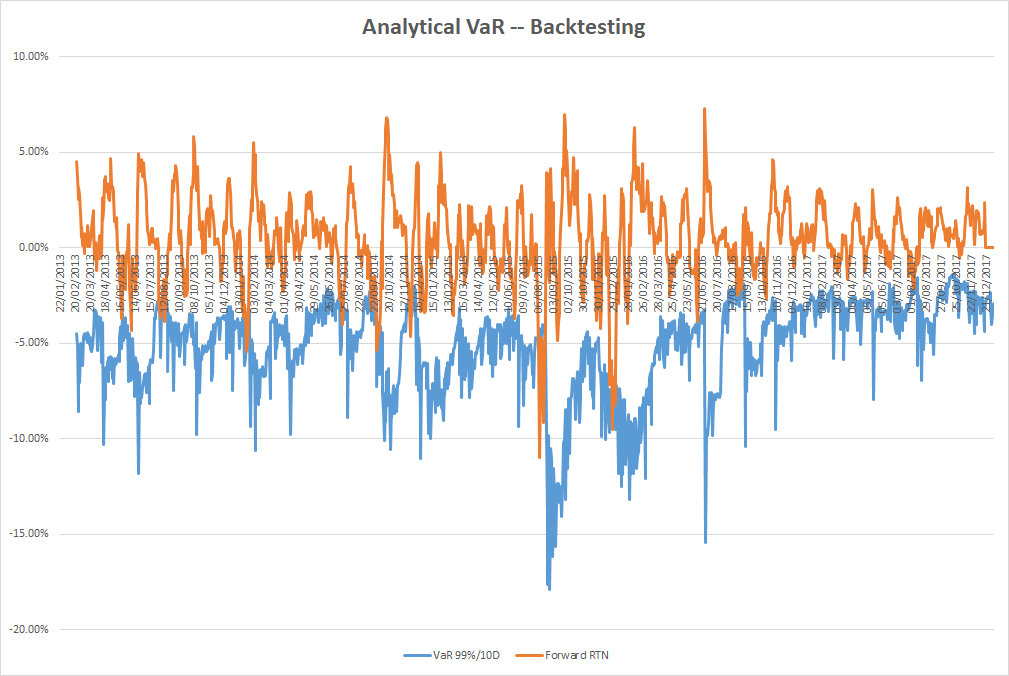
\includegraphics[scale=0.7]{3.2.png}
	      \end{figure}
\end{itemize}

*The calculation process and results are shown in the attached excel file.

\section*{Question 4}
\begin{itemize}

	\item The summary tables is \\
	      \begin{figure}[ht]
		      \centering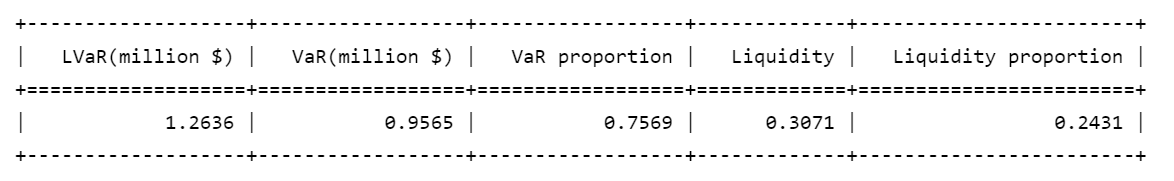
\includegraphics[scale=0.8]{4.1.png}
	      \end{figure}
	\item The summary tables is
	      \begin{figure}[ht]
		      \centering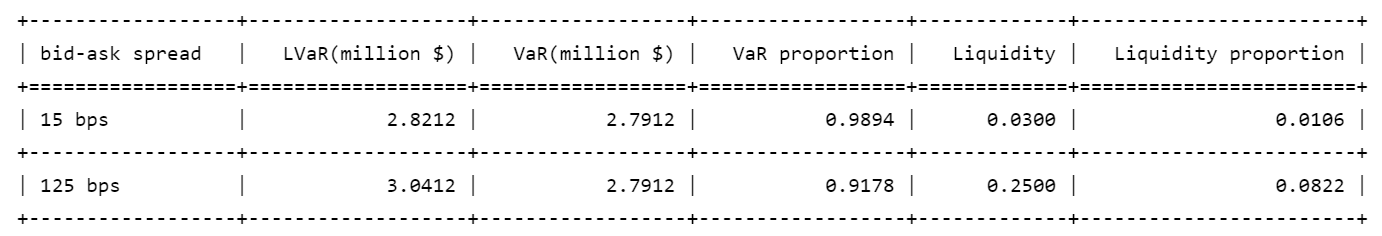
\includegraphics[scale=0.7]{4.2.png}
	      \end{figure}
	      \\
	      If the bid-ask spread increases to 125 bps, the VaR remains unchanged, and the Liquidity increases greatly from 0.0300 to 0.2500, which increases the LVaR from 2.8212 to 3.0412. \\

	      *The calculation process and results are shown in the attached juypter notebook file.

\end{itemize}
\end{document}